% vim: set ts=2 sw=2 noet:

\chapter{Implementation}

\section{Simulaton}
%%TO DO: quelle https://wiki.gnuradio.org/

For the simulation task and after for the Hardware part, the open-source Software GNU Radio has been chosen. This software uses toolboxes for signal processing systems too simulate or/and implement a software-defined radio, based on Python and some C++ implementations for some rapid-application-development environments. The toolboxes can simply, with the help of the graphical user interface, used by drag-and-drop. The Boxes are used to write applications, to receive or to transmit date for a digital system. Some blocks like different filters, channel codes or demodulator elements and a lot more are already implemented. For missing application new elements can be added by coding own block. With the help of the GNU Radio software those toolboxes can easily get connected to each other, creating data streams. 

\begin{figure}
	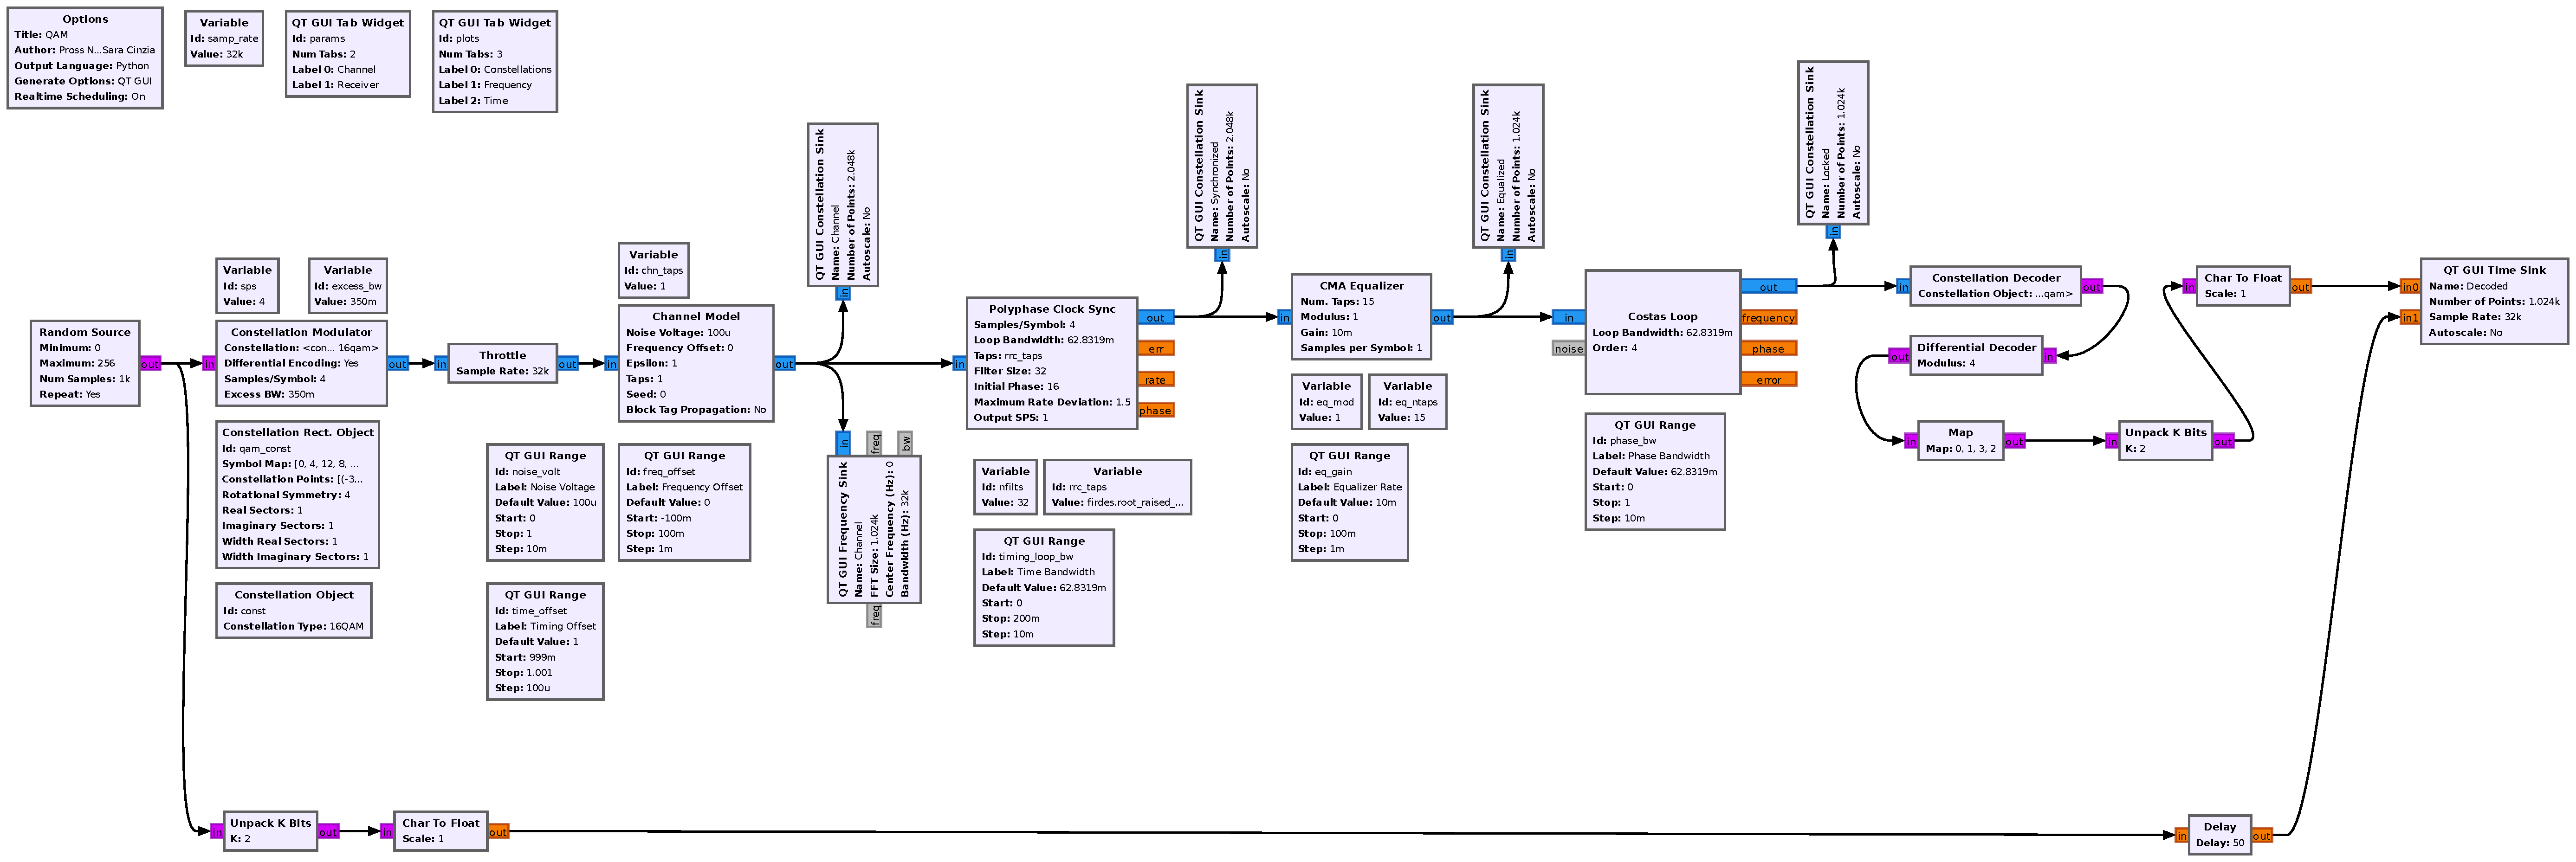
\includegraphics[width=14cm]{./pdfs/qam_nogui.pdf}
	\caption{GNU Radio Blocks}
	\label{fig:simul16QAM_block}	
\end{figure}


\begin{figure}
	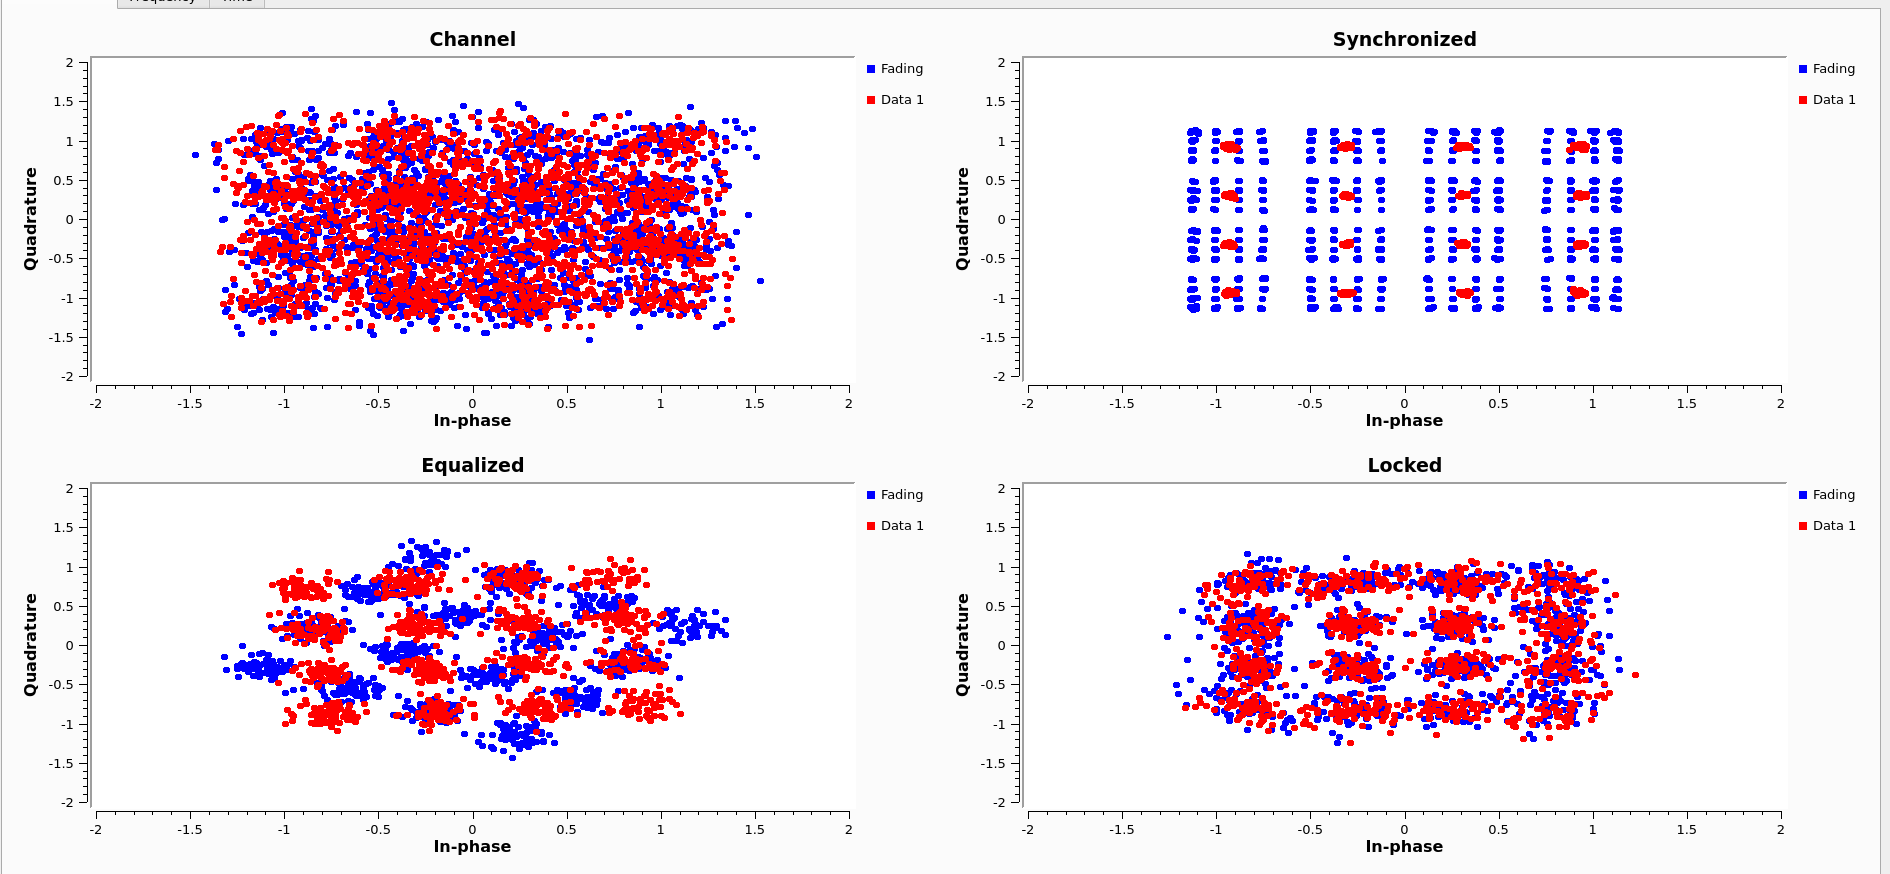
\includegraphics[width=14cm]{./figures/screenshots/QAM16_Fading_2.png}
	\caption{Simulation results}
	\label{fig:simul16QAM}	
\end{figure}

\begin{figure}
	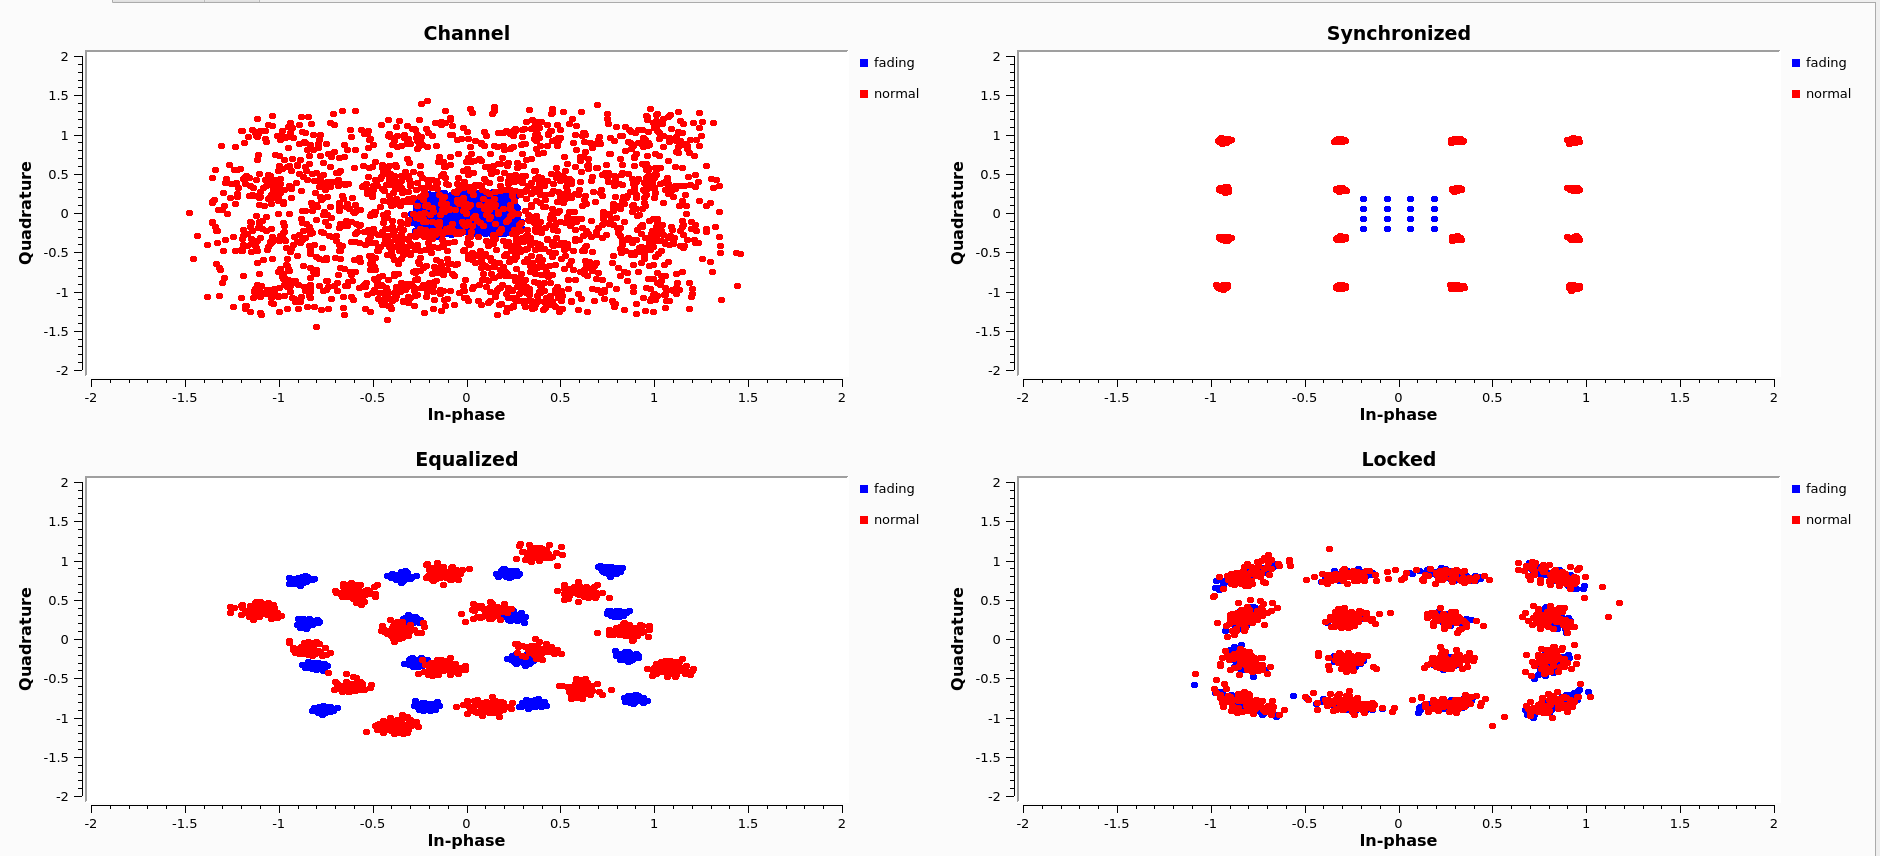
\includegraphics[width=14cm]{./figures/screenshots/QAM16_Fading_2_.png}
	\caption{Simulation results}
	\label{fig:simul16QAM_1}	
\end{figure}

\subsection{16QAM Simulation}
To get a basic line for further simulations a 16QAM has been made. The results of this simulation are shown in \figref{fig:simul16QAM} and \figref{fig:simul16QAM_1} as the red Signal. In \tabref{tab:modulation_settings} some importer Parameter settings for the Simulation Model are mentionet.

\begin{table}[]
	\caption{modulation settings}
	\begin{tabular}[h]{|c|c|c|}
		\hline
		modulation type & Samples per Symbols & costas loop order\\
		\hline
		BPSK & & 2\\
		\hline
		QPSK & & 4\\
		\hline
		8PSK & & 8\\
		\hline 
		16QAM & 4 & 4 \\
		\hline
	\end{tabular}
	\label{tab:modulation_settings}
\end{table}


\subsubsection{Transmitter}
\paragraph{Source}
In this simulation a random source has been chosen.
\paragraph{Modulator}
The constellation modulator block is used for a root-raised-cosine-filtered basis modulation. The block gives an input of a byte stream as complex modulated signal in the baseband back. 
Further more it's possible to chose the modulation type here, in this example it is 16QAM, but QPSK, 8PSK and BPSK would also be possible.

\subsubsection{Channel}
\paragraph{Channel Mode}
Here its possible to add some AWGN noise in the channel line. Different parameters can be changed like the noise voltage, time or the frequency offset.

\subsubsection{Receiver}
\paragraph{Polyphase Clock Sync}
%% To Do : nochmals anschauen ob dieese erklärung verständlich ist und richtig interpretiert wurde.
With the the polyphase clock sync the symbols can be synchronized by preforming a time synchronization with the help of multiple filterbanks. For that the derivation of the filtered signal should be minimized whish turns to a better SNR. This works with the help of two filterbanks, one of them contains the filters of the signal adapted to the pulse shaping with several phases. The other contains its derivative. So in the time domain it has a sinc shape, for the output Signal the sinc peak should be on a sample, with the fact that sinc(0) = 1 and sinc(0)' = 0 an error signal can be generated which tells how far away from the peak it is. This error Signal should be zero this is possible with the help of a loop second order whish constants the number of the filterbank and the rate. This rate is generated because of the clock difference between the transmitter and reviver to synchronies the receiver the filter goes through the phases.

For the output one sample per symbol is enough.

\paragraph{Equalizer}
?


\paragraph{Costas Loop}

The Costas Loop is used for frequency and phase adjustment it locks the center frequency of the signal additional it converts it back to de baseband.  For different modulation types different orders of the loop had to be chosen 

\paragraph{Decoder}

From the complex space the constellation points are decode to bits.



\subsection{Simulation Fading}
For the a first simulation with some fading the 16QAM simulation model has been extended with a FIR-Filter in the Chanel. The results of this simulation are shown in \figref{fig:simul16QAM} and \figref{fig:simul16QAM_1} as the blue Signal.

\subsubsection{Channel}
\subsubsection{FIR-Filter}
A FIR-Filter was added in the Channel to create a time delay between tow paths. In \figref{fig:simul16QAM} the result includes a direct path and a delayed one. In the plot of \figref{fig:simul16QAM_1} the transmission line dosn't include a direct path. It's impotent to mention that the delay should be smaller than the symbol rate or a multiple of it. 


\section{Hardware}

As Hardware we chosen the USRP B210 from Ettus Research, with the following specifications shown in Tab. \ref{tab:USRP B210 specifications}. Because this SDR is more than enough for our requires.

\subsection{Hardware setup}

The First Hardware set up was from the first SDR to the second, with a coaxial cable in between. 
The second was with the antennas. 2.4GHz. 

% To Do: Picture


\begin{table}[]
	%To DO sepzifikationen ampssen / genauer? https://www.ettus.com/wp-content/uploads/2019/01/b200-b210_spec_sheet.pdf
	%https://kb.ettus.com/B200/B210/B200mini/B205mini#FAQ
	\caption{USRP B210 specifications}
	\begin{tabular}[h]{|c|c|}
		\hline
		Dimensions & 9.7 x 15.5 x 1.5 cm \\
		\hline
		Ports &
		2 TX , 2 RX, Half  or Full Duplex\\
		\hline
		RF frequencies & from 70MHz to 6GHz\\
		\hline
		Bandwidth & 200kHz-56MHz\\
		\hline 
		External reference input & 10 MHz \\
		\hline
	\end{tabular}
\label{tab:USRP B210 specifications}
\end{table}


\section{Measurements}



\section{Results}
